\documentclass{book}
\usepackage{amssymb,amsmath}
\usepackage{polyglossia}
\setmainlanguage{spanish} % Idioma principal
\usepackage{theorem}
\usepackage{times}
\usepackage{array}
\usepackage{graphicx}
\usepackage{hyperref}
\usepackage{multirow}
\usepackage{fancyhdr}
%\usepackage[cp1252]{inputenc}
\usepackage{hhline}
\usepackage{multicol}
\usepackage[a4paper,driver=xetex,top=4.5cm,head=4.5cm, bottom=2cm,%
layouthoffset=0mm, left=2.5cm, right=2.5cm,marginparwidth=0cm]{geometry}
%\usepackage{bm}
%\usepackage{tabular}
\usepackage{fontspec}
 \usepackage[breakable,many]{tcolorbox}
\defaultfontfeatures{Ligatures=TeX}
\usepackage{empheq}
 \setromanfont{Roboto Condensed}
 \usepackage{float}
 \usepackage{mathrsfs} 
%
%
% \renewcommand{\familydefault}{\sfdefault}
%\renewcommand{\familydefault}{\sfdefault}

%%%%%%%%%Estilo de la pagina%%%%%%%%%%%%%%%%%%%%%%%%%%%%%%%%%%%
%%%%%%%%%%%%%%%%%%%%%%%%%%%%%%%%%%%%%%%%%%%%%%%%%%%%%%%%%%%%%%%%%%
% \newcounter{ejer}
% 
% {\theorembodyfont{\normalfont}
% \newtheorem{ejercicio}[ejer]{Ejercicio}}

\newcommand{\rr}{\mathbb{R}}
\newcommand{\qq}{\mathbb{Q}}
\newcommand{\nn}{\mathbb{N}}

\newcommand{\di}{\displaystyle}

\DeclareMathOperator{\atan2}{atan2}
%\DeclareMathOperator{\sen}{sen}
\DeclareMathOperator{\sign}{sign}
\DeclareMathOperator{\sn}{sn}
\DeclareMathOperator{\SO}{SO}
%\DeclareMathOperator{\arcsen}{arcsen}
\DeclareMathOperator{\Or}{O}

\usepackage[framemethod=TikZ]{mdframed}
%%%%%%%%%%%%%%%%%%%%%%%%%%%%%%
%Theorem

%% Ejercicio
\newcounter{ejer} \setcounter{ejer}{0}
\renewcommand{\theejer}{\arabic{ejer}}
\newenvironment{ejer}[2][]{%
\vspace{5pt}
\refstepcounter{ejer}%
\ifstrempty{#1}%
{%
% \mdfsetup{%
% frametitle={%
% \tikz[baseline=(current bounding box.east),outer sep=-0pt]
% \node[anchor=east,rectangle,fill=green!50]
{\noindent\bfseries Ejercicio~\theejer}.}
%
{%
% \mdfsetup{%
% frametitle={%
% \tikz[baseline=(current bounding box.east),outer sep=0pt]
% \node[anchor=east,rectangle,fill=green!50]
{\noindent\bfseries  Ejercicio~\theejer:~#1};}%
%
%\mdfsetup{innertopmargin=10pt,linecolor=green!50,%
%linewidth=2pt,topline=true,%
%frametitleaboveskip=\dimexpr-\ht\strutbox\relax
%}
%\begin{mdframed}[]
\relax%
\label{#2}}{\vspace{5pt}}%\end{mdframed}}

%Theorem
\newcounter{theo}[chapter] \setcounter{theo}{0}
\renewcommand{\thetheo}{\arabic{section}.\arabic{theo}}
\newenvironment{theo}[2][]{%
\refstepcounter{theo}%
\ifstrempty{#1}%
{\mdfsetup{%
frametitle={%
\tikz[baseline=(current bounding box.east),outer sep=0pt]
\node[anchor=east,rectangle,fill=blue!20]
{\strut Teorema~\thetheo};}}
}%
{\mdfsetup{%
frametitle={%
\tikz[baseline=(current bounding box.east),outer sep=0pt]
\node[anchor=east,rectangle,fill=blue!20]
{\strut Teorema~\thetheo:~#1};}}%
}%
\mdfsetup{innertopmargin=10pt,linecolor=blue!20,%
linewidth=2pt,topline=true,%
frametitleaboveskip=\dimexpr-\ht\strutbox\relax
}
\begin{mdframed}[]\relax%
\label{#2}}{\end{mdframed}}
%%%%%%%%%%%%%%%%%%%%%%%%%%%%%%
%Lemma
\newcounter{lem}[chapter] \setcounter{lem}{0}
\renewcommand{\thelem}{\arabic{section}.\arabic{lem}}
\newenvironment{lem}[2][]{%
\refstepcounter{lem}%
\ifstrempty{#1}%
{\mdfsetup{%
frametitle={%
\tikz[baseline=(current bounding box.east),outer sep=0pt]
\node[anchor=east,rectangle,fill=green!20]
{\strut Lemma~\thelem};}}
}%
{\mdfsetup{%
frametitle={%
\tikz[baseline=(current bounding box.east),outer sep=0pt]
\node[anchor=east,rectangle,fill=green!20]
{\strut Lemma~\thelem:~#1};}}%
}%
\mdfsetup{innertopmargin=10pt,linecolor=green!20,%
linewidth=2pt,topline=true,%
frametitleaboveskip=\dimexpr-\ht\strutbox\relax
}
\begin{mdframed}[]\relax%
\label{#2}}{\end{mdframed}}
%%%%%%%%%%%%%%%%%%%%%%%%%%%%%%
%% Definicion
\newcounter{defini}[chapter] \setcounter{defini}{1}
\renewcommand{\thedefini}{\arabic{section}.\arabic{defini}}
\newenvironment{definicion}[2][]{%
\refstepcounter{defini}%
\ifstrempty{#1}%
{\mdfsetup{%
frametitle={%
\tikz[baseline=(current bounding box.east),outer sep=0pt]
\node[anchor=east,rectangle,fill=green!20]
{\strut Definición~\thedefini};}}
}%
{\mdfsetup{%
frametitle={%
\tikz[baseline=(current bounding box.east),outer sep=0pt]
\node[anchor=east,rectangle,fill=green!20]
{\strut Definición~\thedefini:~#1};}}%
}%
\mdfsetup{innertopmargin=10pt,linecolor=green!20,%
linewidth=2pt,topline=true,%
frametitleaboveskip=\dimexpr-\ht\strutbox\relax
}
\begin{mdframed}[]\relax%
\label{#2}}{\end{mdframed}}

%Proof
\newenvironment{prf}{\noindent\emph{Dem.}}{$\square$ \newline\vspace{5pt}}


%Corolario
\newcounter{cor}[chapter] \setcounter{cor}{0}
\renewcommand{\thecor}{\arabic{section}.\arabic{cor}}
\newenvironment{cor}[2][]{%
\refstepcounter{cor}%
\ifstrempty{#1}%
{\mdfsetup{%
frametitle={%
\tikz[baseline=(current bounding box.east),outer sep=0pt]
\node[anchor=east,rectangle,fill=green!20]
{\strut Corolario~\thelem};}}
}%
{\mdfsetup{%
frametitle={%
\tikz[baseline=(current bounding box.east),outer sep=0pt]
\node[anchor=east,rectangle,fill=green!20]
{\strut Corolario~\thelem:~#1};}}%
}%
\mdfsetup{innertopmargin=10pt,linecolor=green!20,%
linewidth=2pt,topline=true,%
frametitleaboveskip=\dimexpr-\ht\strutbox\relax
}
\begin{mdframed}[]\relax%
\label{#2}}{\end{mdframed}}

\tcbset{highlight math style={enhanced,
  colframe=red!60!black,colback=yellow!50!white,arc=4pt,boxrule=1pt,
  drop fuzzy shadow}}
  
  
  
  
  
  
  


\pagestyle{fancyplain}

 \renewcommand{\sectionmark}[1]
                 {\markright{\thesection\ #1}}


% \lhead[\fancyplain{}{\bfseries\thepage}]
%       {\fancyplain{}{\bfseries\rightmark}}
%
 \rhead[\fancyplain{}{\bfseries\leftmark}]{\fancyplain{}{\bfseries}}




 \lhead[\fancyplain{}{ 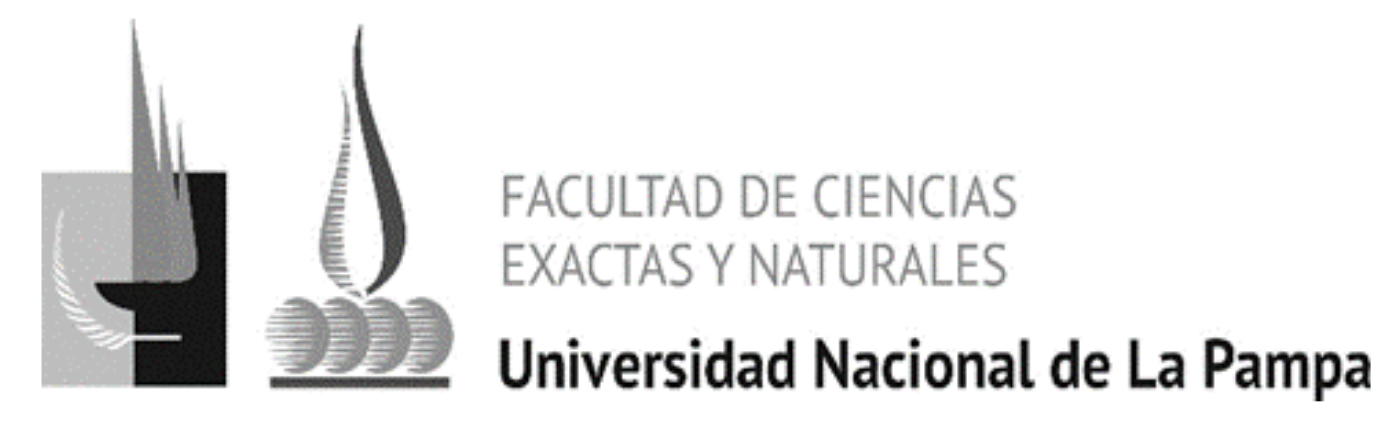
\includegraphics[scale=.3]{EscudoUNLPam.png}}]{\fancyplain{}{ 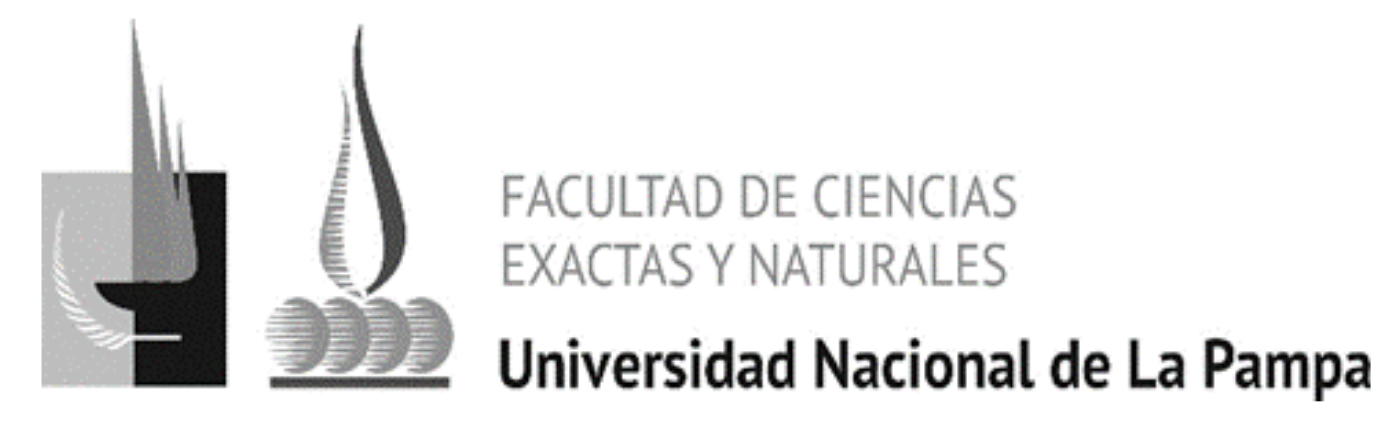
\includegraphics[scale=.3]{EscudoUNLPam.png}}}

\cfoot{}





  
  
  
  
  
  
  
\begin{document}


\hyphenation{excen-tri-ci-dad}


\begin{large}
\begin{bfseries} % \begin{scshape}
        \noindent Depto de Matem\'atica.\\
        Primer Cuatrimestre de 2022\\                                                                                                                                                                                                                                                                                                                                                
        Teoría de la Medida \\
        Práctica 3: Medida de Lebesgue

%\end{scshape}
\end{bfseries}
\end{large}
\par\noindent\rule{\textwidth}{.5pt}









\begin{ejer}{} Sean $R$ y $R_j$, $j=1,\ldots,M$, rectángulos de  $\rr^d$ con $R\subset \bigcup\limits_{j=1}^M R_j$. 
 Probar que $|R|\leq \sum\limits_{j=1}^N |R_j|$, 
 donde $|R|$ es el volumen del rect\'angulo $R$ y 
 $|R_j|$ es el volumen de cada  rect\'angulo $R_j$ para $j=1,2,\ldots,M.$
\end{ejer}


\begin{ejer}{}  Demostrar que  $m_*(A)=0$  cuando $A\subset\mathbb{R}^d$ es numerable.
\end{ejer}  

%\begin{ejer}{} Probar que
%\begin{enumerate}
%\item Si $m_*$ fuera finitamente %aditiva, entonces $m_*$ sería  %sigma aditiva.
%\item Si $m_*(A)=0$, entonces $m_*(A\cup B)=m_*(A)+m_*(B)=m_*(B)$.
%\end{enumerate}
%\end{ejer} 









 




 \begin{ejer}{}
	Mostrar que cualquier conjunto con medida exterior positiva contiene un conjunto acotado con medida exterior positiva. 
	\end{ejer}
 
  \begin{ejer}{} 
	Probar que si $m_*(E)>0$ y $0<\alpha<1$, entonces existe un cubo $Q$, tal que
  $m_*(E\cap Q)>\alpha m(Q)$.
\\
  \underline{Sugerencia:} suponiendo primero que $0<m_*(E)<\infty$, considerar un conjunto
 $U=\di\bigcup_{k=1}^{\infty}Q_k$, tal que 
  $U\supset E$ y $\sum\limits_{k=1}^{\infty}m(Q_k)<\alpha^{-1} m_*(E)$; entonces al menos uno de los cubos $Q_k$
  debe satisfacer la desigualdad del enunciado.
 \end{ejer} 

\begin{ejer}{}
  En la teoría se demostró que el disco abierto  de $\rr^2$ definido por  $x^2+y^2< 1$ se puede escribir como una unión numerable de cubos casi-disjuntos. Demostrar que esta afirmación es falsa si consideramos el disco cerrado  $x^2+y^2\leq 1$.  
	\end{ejer}






  \begin{ejer} {} 
	{\it{Decimos que un conjunto $E\subset \rr^d$ 
  {\bf{satisface la condición de Caratheodory}}
  si para cualquier conjunto $S\subset \rr^d$ se verifica}} 
  $$m_*(S\cap E)+m_*(S-E)=m_*(S). $$
%%%%%%%%%%%%%%
	\begin{enumerate}   
    \item Probar que todo conjunto medible $E$ satisface la condición de Caratheodory.
    \\
    \underline{Sugerencia:} basta probar que para cualquier conjunto $S$ se cumple
    $$m_*(S\cap E)+m_*(S-E)\leq m_*(S), $$
    en vista de que la desigualdad opuesta se cumple en cualquier caso.
 
    \item Probar que si $E_1$ y $E_2$ satisfacen la condición de Caratheodory, 
    entonces la intersección de ambos conjuntos también la satisface.
    \\
    \underline{Sugerencia:} el conjunto $S-E_1\cap E_2$ es la unión de los conjuntos 
    disjuntos $S\cap E_1-E_2$, $(S-E_1)\cap E_2$ y $(S-E_1)-E_2$.

    \item Probar que si $E$ satisface la condición de Caratheodory, entonces $E$ es medible.
    \\
    \underline{Sugerencia:} en virtud de los incisos  1. y  2. se puede suponer que $E$ es acotado.
	\end{enumerate}
    La moraleja del problema es que 
    %%%% 
    {\bf{``los conjuntos medibles son exactamente los que satisfacen
    la condición de Caratheodory.''}}
  \end{ejer} 
	
	
 

%  \begin{ejer} {}
 % Si el conjunto $E$ es la unión de una sucesión creciente de conjuntos 
  %$E_1\subset E_2\subset E_3\subset...$, entonces 
  %$ m_e(E)=\di\lim_{k\rightarro%w \infty} m_e(E_k).$
  %\\
  %\underline{Sugerencia:} para %cada $k$ elíjase un conjunto %$H_k$ de clase $G_{\delta}$,
  %tal que $E_k\subset H_k$, $m(H_k)=m_e(E_k)$; los conjuntos de clase $G_{\delta}$
  %$$D_k=H_k\cap H_{k+1}\cap H_{k+2}\cap... $$
  %para $k=1,2,3,...$ forman una sucesión creciente que verifica %$E_k \subset D_k$,
  %$m(D_k)=m_e(E_k)$ y el conjunto $E$ está incluido en la unión %de los $D_k$, de donde
  %se sigue que $m_e(E)\leq \di\lim_{k\rightarrow \infty} %m_e(E_k)$.
  %\\
  %La desigualdad opuesta es inmediata.
 %\end{ejer}



 \begin{ejer}{}
	 Para cualquier conjunto $E \subset \rr^d$,  probar que: 
	\begin{enumerate}
	    \item 
	    \label{ej-guia}
existe un conjunto $H$ de clase $G_{\delta}$,
  tal que $E \subset H$ y $m_*(E)=m(H)$.
  \item 
  existe un conjunto $H$ de
  clase $G_{\delta}$, tal que $E \subset H$ y para cualquier conjunto medible $M$ se cumple
  $$m_*(E \cap M)=m(H\cap M).$$
  %%
  \underline{Sugerencia:} suponiendo primero que $m_*(E)<\infty$, considérese un conjunto
  $H$ de clase $G_{\delta}$ como en el inciso \ref{ej-guia}. El conjunto $M$ satisface la
  condición de Caratheodory con respecto a $E$.
  	\end{enumerate}
	
  \end{ejer} 

   \begin{ejer}{}
	Probar que si $E_1$ y $E_2$ son conjuntos medibles disjuntos, entonces para cualquier
  conjunto $S \subset \rr^d$ se cumple 
  $$m_*(S\cap E_1)+m_*(S\cap E_2)=m_*(S\cap(E_1\cup E_2)). $$
  Generalizar a cualquier sucesión $(E_k)$ de conjuntos medibles disjuntos.
   \end{ejer} 


	 \begin{ejer}{} 
 Si $E$ y $F$ son conjuntos medibles cualesquiera, entonces
  $$m(E \cup F)+m(E \cap F)=m(E)+m(F).$$
	\end{ejer} 


   \begin{ejer}{}  Probar que $G \in G_{\delta}$ si y sólo si $G^c \in F_{\sigma}$.
\end{ejer} 
 
%

%\begin{ejer}{} 
 %Sea $E$ un conjunto medible %Lebesgue con $m(E)<\infty$.
%\\Probar que existe una sucesi\'on %decreciente de conjuntos abiertos %$(G_k)$ tal que
%$\lim m(G_k)=m (E)$.
%\end{ejer} 



%\begin{ejer}{}*
 %Sea  $E$ un conjunto medible %Lebesgue con $m(E)<\infty$.\\
%Probar que existe una sucesi\'on %creciente de conjuntos cerrados %$(F_k)$ tal que
%$\lim m(F_k)=m (E)$.
%\end{ejer} 

    \begin{ejer}{} 
	Probar que para cualquier conjunto medible $E$ vale la fórmula
   $$m(E)=\sup\{m(K):K\subset E\}, $$
   donde el supremo se toma sobre todos los conjuntos compactos $K \subset E$.
\end{ejer} 

   \begin{ejer}{} 
	Sea $(E_k)$ una sucesión de conjuntos medibles. Probar que
	\begin{enumerate}
    \item $m(\liminf E_k)\leq \liminf m(E_k)$;
    \item si para alg\'un $j$, \;$m\left(\di\bigcup_{k\geq j}E_k\right)<\infty$, luego\; 
    $\limsup m(E_k)\leq m(\limsup E_k)$;
    \item si la sucesión $(E_k)$ tiende a un límite y todos los $E_k$ son subconjuntos
    de un conjunto fijo $A$ de medida finita, entonces \;$m(\lim E_k)=\lim m(E_k)$.
    \item
    Exhibir una sucesión de conjuntos $E_k$ en el intervalo unitario $[0,1]$, tal que 
    $m(\liminf E_k)<\liminf m(E_k)<\limsup m(E_k)<m(\limsup E_k)$  (todas las desigualdades estrictas).
	\end{enumerate}
	\end{ejer} 

   \begin{ejer}{} 
	Mostrar que existe un conjunto $H$ incluido en el intervalo unitario $[0,1]$, de clase
  $F_{\sigma}$, de medida uno, formado exclusivamente por puntos irracionales. 
  \\
  Mostrar que $H$ es unión numerable de conjuntos cerrados con interior vacío.
\end{ejer} 

 \begin{ejer}{}  * 	Demostrar que $\mathscr{O}$ es $\sigma$-álgebra si:
	\[\mathscr{O}=\{Z\subset \Omega|\,m(Z)=0 \;\;\text{ó}\;\; m(Z^c)=0\}.
	\]
	\end{ejer} 


\begin{ejer}{} 
Mostrar que el conjunto $\mathscr{O}=\{G|\; G \text{ es un conjunto abierto o cerrado de } \mathbb{R}\}$ no es una $\sigma$-álgebra. 
\end{ejer} 


\begin{ejer}{} 
Si $(A_k)$ es una sucesi\'on de conjuntos en una $\sigma$-\'algebra $\mathscr{O}$, entonces
\begin{enumerate}
%\item $\bigcap A_k$ pertenece a la $\sigma$-\'algebra $\mathscr{O}$.
\item $\limsup A_k=\bigcap\limits_{k\geq 1}\left(\bigcup\limits_{n\geq k} A_n\right)$ pertenece a $\mathscr{O}$.
\item * $\liminf A_k=\bigcup\limits_{k\geq 1}\left(\bigcap\limits_{n\geq k} A_n\right)$ pertenece a $\mathscr{O}$.
 \end{enumerate}
 \end{ejer}  





\begin{ejer}{} 
Sea $f: A\to B$ una funci\'on.  
\begin{enumerate}
    \item  Sup\'ongase 
$\mathscr{O}_2$ es una $\sigma$-\'algebra en $B$.  Probar que el conjunto de im\'agenes inversas de los conjuntos en $\mathscr{O}_2$  forman una 
$\sigma$-\'algebra en $A$. 
\item Sup\'ongase que  $\mathscr{O}_1$ es una $\sigma$-\'algebra en $A$.
Probar que los conjuntos de $B$ cuyas im\'agenes inversas pertenecen a $\mathscr{O}_1$ forman una 
$\sigma$-\'algebra en $B$. 
\end{enumerate}
Probar que el conjunto de im\'agenes inversas de los conjuntos en $\mathscr{O}$  forman una 
$\sigma$-\'algebra en $A$. 
\end{ejer}


  

	\begin{ejer}{} Demostrar que si $A,B$ son borelianos de $\rr$ entonces $A\times B$ es boreliano de $\rr^2$. 
	 	\end{ejer}




%\begin{ejer}{}* Probar que $\sqrt{2}$ no es %equivalente a $\sqrt{3}$ respecto a la %relación definida para la construcción del %conjunto de Vitali.
%\end{ejer}
  
  
   \begin{ejer}{} 
	?`Cómo son los subconjuntos medibles del conjunto de Vitali?
\end{ejer} 


\end{document}
